\section{Результати роботи програми}

Для верифікації правильності роботи розроблених алгоритмів було здійснено запуск програми в 
єдиному циклі збирання середовища VS Code. На рисунку~\ref{fig:terminal} представлено фінальне 
виведення результатів у термінал Windows PowerShell.

\begin{figure}[H]
    \centering
    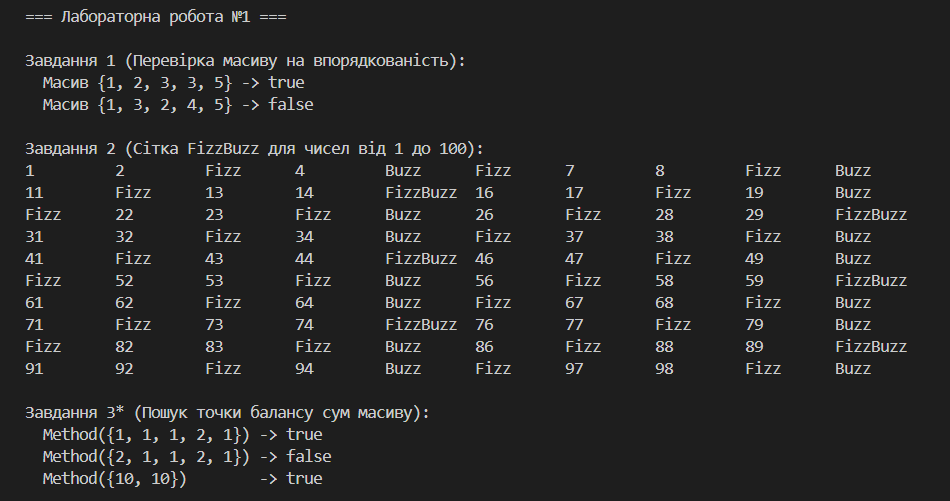
\includegraphics[width=0.95\textwidth]{screenshots/terminal_output.png}
    \caption{Вигляд терміналу після успішного виконання всіх трьох завдань лабораторної роботи}
    \label{fig:terminal}
\end{figure}

Як видно з результатів тестування:
\begin{itemize}
    \item 
    Компонент \texttt{ArrayChecker} коректно визначив впорядкованість першого 
    масиву (\texttt{true}) та зафіксував порушення порядку у другому (\texttt{false}).
    \item 
    Гра \texttt{FizzBuzzGame} згенерувала компактну текстову матрицю 
    розміром $10 \times 10$ елементів із правильним заміщенням чисел на відповідні мовні маркери.
    \item 
    Оптимізований обчислювач \texttt{BalanceFinder} безпомилково знайшов точки 
    рівноваги сум для демонстраційних масивів.
\end{itemize}
